\subsection{Implementing an IPython kernel for Jupyter notebooks}
\label{sec:literate-programming}

As explained in \cref{sec:a-literate-programming}, IPython (together with
Jupyter notebooks) supports both reproducible research and literate
programming. The client had expressed his interest in literate programming
functionality for Spoofax. Implementing an IPython kernel on top of the core
shell module should not take a lot of effort, however due to the problems
discussed earlier priority was given to a solid working REPL and an Eclipse
plugin. Therefore our product does not deliver an implementation of literate
programming.

IPython kernels provide a solid framework for literate programming that has
proven itself in many different languages
\footnote{https://github.com/ipython/ipython/wiki/IPython-kernels-for-other-languages}.
An IPython kernel is basically a daemon with several network sockets
representing the in and output streams of the client application. Several
message types are sent over these sockets in JSON format, such as requests to
evaluate a certain string or requests regarding the kernel
state\footnote{https://jupyter-client.readthedocs.io/en/latest/kernels.html}.

Since the invoker class from the core module just accepts any string given to
it and then resolves the command itself, implementing an IPython kernel should
be pretty straightforward. Most of the required work would be in creating an
adequate messaging framework capable of understanding all defined JSON
messages. When the messaging framework is in place user input can be sent
directly to the invoker and results can be displayed using the ``IResult''
interfaces as with any other client implementation.

\begin{figure}[htb]
  \centering
  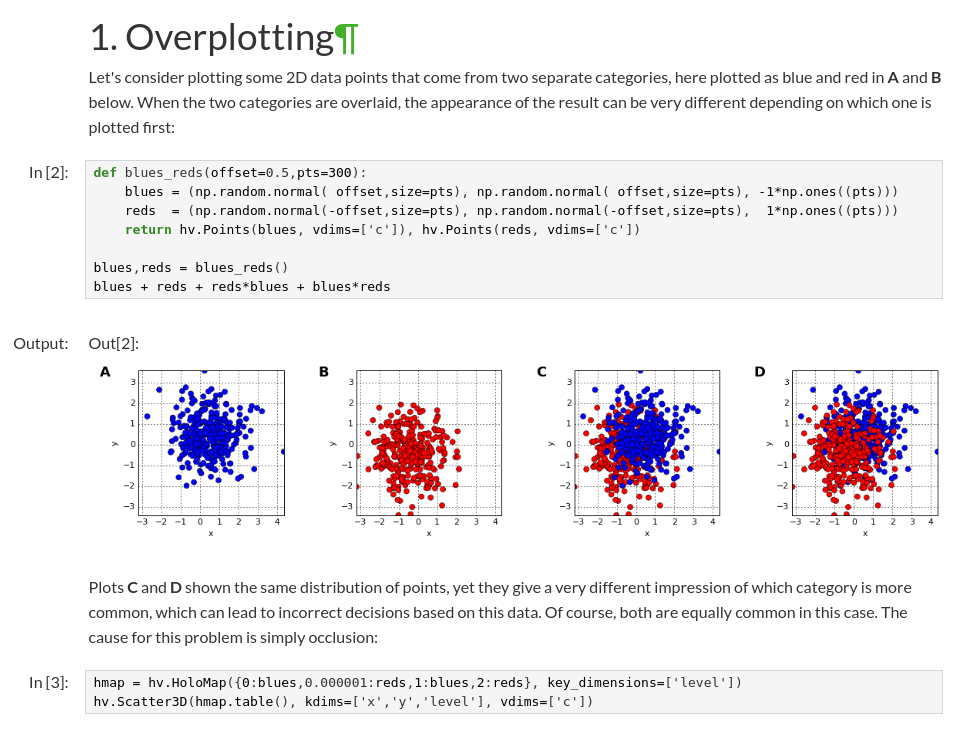
\includegraphics[width=\textwidth]{ipython}
  \caption{A plot from data in an IPython notebook.}
  \label{fig:ipython}
\end{figure}

By implementing an IPython kernel all functionality offered by Jupyter
notebooks (see \cref{fig:ipython}) would be available to the Spoofax REPL at
once. This would directly result in the ability to live edit code interspersed
with documentation, while also allowing more complex graphical elements.

%%% Local Variables:
%%% mode: latex
%%% TeX-master: "../main"
%%% End:
